\documentclass[11pt, oneside, a4paper]{article}
%\usepackage[cp1251]{inputenc} % кодировка
\usepackage[utf8]{inputenc} % кодировка
\usepackage[english, russian]{babel} % Русские и английские переносы
\usepackage{graphicx}          % для включения графических изображений
\usepackage{cite}              % для корректного оформления литературы
\usepackage{enumitem}
\usepackage{pavt-ru}  
\usepackage{amsmath} 
\usepackage{graphicx}
\graphicspath{{pictures/}}
\DeclareGraphicsExtensions{.pdf,.png,.jpg}
                           

\begin{document}

% \title - название статьи
% \authors - список авторов

\title{Оптимизация алгоритмов сжатия цифровых сигналов на системах с общей памятью}

\authors{А.В.~Данилова\superscript{1}, Н.В.~Пауков\superscript{1}, М.А.~Теплякова\superscript{1}}
\organizations{\superscript{1}Воронежский государственный университет}

% Аннотация заключается в окружение abstract
\begin{abstract}
В данной работе была рассмотрена задача поиска оптимального алгоритма сжатия, соответствующего классу сигналов конкретного типа. С этой целью был разработан алгоритм перебора преобразований сигнала, для реализации которого используются ресурсы суперкомпьютерного центра ВГУ.
\end{abstract}

\keywords{сжатие сигналов, параллельное программирование, дискретное преобразование Фурье.}

% \section{название} - заголовок раздела первого уровня
% \subsection{название} - заголовок раздела второго уровня
% \subsubsection{название} - заголовок раздела третьего уровня
% Не используйте уровень вложенности заголовков больше трех!
% Каждый абзац текста в статье начинается командой \par или пустой
% строкой.

\section{Введение}

В настоящее время создание новых методов и алгоритмов обработки цифровых сигналов является перспективной и крайне важной областью научных исследований. Первой ключевой задачей в этом направлении является очистка сигнала от постороннего шума, появляющегося в результате неточных измерений, фоновых помех или неисправности аппаратуры. Также стоит отметить тот факт, что большую практическую значимость имеют методы сжатия, основная идея которых в том, чтобы сохранить всю важную информацию, присутствующую в сигнале, сократив при этом объём памяти, используемый для её хранения.

Многие способы сжатия основаны на использовании дискретного преобразования Фурье (ДПФ), поскольку оно оказывается эффективным для широкого спектра сигналов [1, 2]. ДПФ используется в реализации многих методов сжатия изображения и видео, таких как JPEG, MPEG и прочих. Также в настоящее время для цифровой обработки сигналов активно используются вейвлеты различных типов [3, 4].

Существенным аспектом является тот факт, что для сигналов разной структуры эффективнее оказываются те или иные конкретные методы. По этой причине развитие получила область исследований, связанная с разработкой адаптивных алгоритмов. Один из основных подходов в этом направлении состоит в выборе некоторого класса функций, имеющего набор подстраиваемых параметров. Чаще всего для этих целей используют различные модификации вейвлетов [5, 6]. 

Затем для конкретных наборов сигналов параметры подбираются таким образом, чтобы повысить эффективность сжатия: максимальное уменьшение объема памяти при сохранении значимой информации. 
Недостатком такого подхода является то, что на данный момент существует множество вейвлетов и выбор какого-то конкретного их вида далеко не очевиден. Кроме того, для некоторых сигналов эффективнее может оказаться использование более простых математических методов, например, функции Гаусса для электрокардиограмм [7, 8].

Следовательно, разработка алгоритмов автоматического отыскания оптимального способа сжатия для определенного типа сигналов представляет серьёзный практический интерес. 

При наличии значительных вычислительных ресурсов, указанную выше задачу можно было бы решить простым перебором различных способов преобразования сигнала, но в реальных условиях это заняло бы слишком большое количество времени. Помимо этого, немаловажно чётко определить то, какие методы сжатия мы будем считать оптимальными. Таким образом, что касается конкретных задач, то стоит отметить следующие:
\begin{itemize}
\item выбор критерия для определения оптимальности конкретных способов сжатия;
\item создание эффективного алгоритма для поиска оптимальных методов сжатия.
\end{itemize}

Так как задачи оптимизации с большими объемами данных являются весьма  ресурсозатратными, то для реализации поставленной цели было принято решение использовать алгоритмы параллельного программирования для систем с общей памятью. Для реализации вычислительных алгоритмов был выбран один из самых распространенных стандартов программирования систем с общей памятью OpenMP. Расчеты производились с использованием ресурсов Суперкомпьютерного центра Воронежского государственного университета.

\section{Методика расчётов}

Рассмотрим цифровой сигнал как некоторый вектор $F$. Тогда, как правило, все методы сжатия устроены следующим образом.

\subsection{Анализ} 

К рассматриваемому сигналу применяется некоторое невырожденное линейное преобразование
\begin{equation}
\label{directConverstion}
    G = T^{-1} F
\end{equation}
где $G$ - преобразованный сигнал, $T$ - матрица преобразования, $T^{-1}$ - обратная матрица. В дальнейшем мы будем использовать краткое обозначение $S = T^{-1}$.

\subsection{Непосредственно сжатие} 

Сигнал $G$ подвергают каким-либо изменениям. В задачах сжатия обычно наименьшие по модулю компоненты $G$ полагают равными нулю. Полученный после этого вектор $\tilde{G}$ сохраняют, и он занимает в памяти меньше места, чем $G$. Процентное отношение количества компонент, которые были отброшены, к общей длине вектора $G$ будем называть уровнем сжатия.

\subsection{Синтез} 

К вектору $\tilde{G}$ применяется обратное преобразование 
\begin{equation}
\label{inverseConverstion}
    \tilde{F} = T\tilde{G}
\end{equation}
где $\tilde{F}$ – восстановленный сигнал. Очевидно, если сжатие не производилось $G=\tilde{G}$, то восстановленный сигнал (без учета погрешности вычислений) совпадает с исходным $F=\tilde{F}$. В общем случае $F$ и $\tilde{F}$ будут отличаться, и допустимым является уровень сжатия, при котором их различия не будут затрагивать полезную часть информации.

Приемлемое значение отклонения восстановленного сигнала от исходного зависит от конкретной задачи, которую решает исследователь. В данной работе для оценки степени соответствия $F$ и $\tilde{F}$ был применен широко используемый общий параметр – отклонение по среднеквадратичной норме $\sigma$:
\begin{equation}
\label{squareNorm}
    \sigma = ||F-\tilde{F}||=\sqrt{\frac{\sum\limits_{k=0}^{n}(f_k-\tilde{f_k})^2}{n+1}}
\end{equation}
где $n+1$ – длина векторов $F$ и $\tilde{F}$, $f_k$ и $\tilde{f_k}$ – их компоненты. Оптимальной будем считать матрицу преобразования $S$, имеющую при заданном уровне сжатия среднюю ошибку $\sigma$ меньшую, чем ДПФ, или же близкую к нему.

Для расчетов использовалось дискретное косинусное преобразование Фурье, заданное следующим образом [5]
\begin{equation}
\label{DCT}
\hat{f_m}=\frac{1}{\sqrt{2n+1}}(f_0+2\sum\limits_{k=1}^{n}f_k\cos(\frac{2 \pi k m}{2n+1})), m=0,1,...,n.
\end{equation}
Формула обращения тогда имеет вид
\begin{equation}
\label{inverseDCT}
f_k=\frac{1}{\sqrt{2n+1}}(\hat{f_0}+2\sum\limits_{m=1}^{n}\hat{f_m}\cos(\frac{2 \pi k m}{2n+1})), k=0,1,...,n.
\end{equation}
Данному преобразованию соответствует следующая матрица
\begin{equation}
\label{matrixDCT}
S = \frac{1}{\sqrt{2n+1}}\begin{pmatrix}
1 & 2 & 2 & \ldots & 2\\
1 & 2\cos\frac{2 \pi}{2n+1} & 2\cos\frac{4 \pi}{2n+1} & \ldots & 2\cos\frac{2 \pi n}{2n+1}\\
1 & 2\cos\frac{4 \pi}{2n+1} & 2\cos\frac{8 \pi}{2n+1} & \ldots & 2\cos\frac{4 \pi n}{2n+1}\\
\vdots & \vdots & \ddots & \vdots\\
1 & 2\cos\frac{2 \pi n}{2n+1} & 2\cos\frac{4 \pi n}{2n+1} & \ldots & 2\cos\frac{2 \pi n^2}{2n+1}
\end{pmatrix}
\end{equation}
Как видим, в данном случае $S=T^{-1}=T$

\section{Структура алгоритма поиска оптимального преобразования}

Ключевым этапом алгоритма поиска оптимального метода сжатия является генерация исследуемого набора матриц преобразования. Во время поиска оптимальной матрицы среди исследуемого набора возникает необходимость в хранении информации о рассматриваемых матрицах. При этом нужно                   учитывать аппаратные ограничения используемого для расчётов вычислительного устройства, так как в данном случае особенности работы с памятью существенно влияют на построение алгоритма. С целью уменьшения количества матриц, единовременно хранящихся в памяти устройства, был рассмотрен следующий вариант алгоритма генерации матриц преобразования и поиска наиболее эффективной матрицы.

В качестве возможных значений элементов матрицы были выбраны числа $1, -1$ и $0$. При этом максимальное количество матриц, полученное вариацией значений элементов, было бы равно $3^{(n+1)^2}$. Для уменьшения объема вычислений было решено организовать строгую классификацию генерируемых матриц, которая бы позволила избежать одновременного хранения всего исследуемого спектра матриц. Данная классификация должна отражать степень эффективности матриц преобразования, а также их элементный состав. Было решено разбить матрицы на классы по количеству входящих в них элементов, имеющих значение $1$. После нахождения наиболее оптимального класса матриц, его также разбить на подклассы по количеству элементов, имеющих значение $-1$.

Но даже после выделения этой группы матриц, предположительно обладающих высокой эффективностью для сжатия рассматриваемой группы сигналов, выбранные матрицы всё ещё являются слишком разнородными и, следовательно, нельзя утверждать, что они обладают одинаковой эффективностью сжатия. Для того чтобы разрешить эту проблему, можно провести дальнейшую классификацию матриц, учитывающую количество элементов со значениями $1$ и $-1$ по строкам, а также их взаимное месторасположение. 

Однако подобное разбиение матриц преобразования на классы не позволяет учесть случайных факторов, влияющих на эффективность преобразования. Кроме того, нельзя утверждать, что матрицы, составленные из элементов, имеющих ограниченный дискретный набор значений, подходят для решения поставленной задачи. Вследствие этого было решено отказаться от описанного ранее алгоритма. Вместо него использовался представленный далее алгоритм, созданный с учётом вышеозначенных идей.

\section{Алгоритм поиска оптимального преобразования}

В данном исследовании расчеты были построены по итерационному принципу. Схема предложенного алгоритма показана на рис. \ref{block-diagram}.

\begin{figure}[h]
	\center{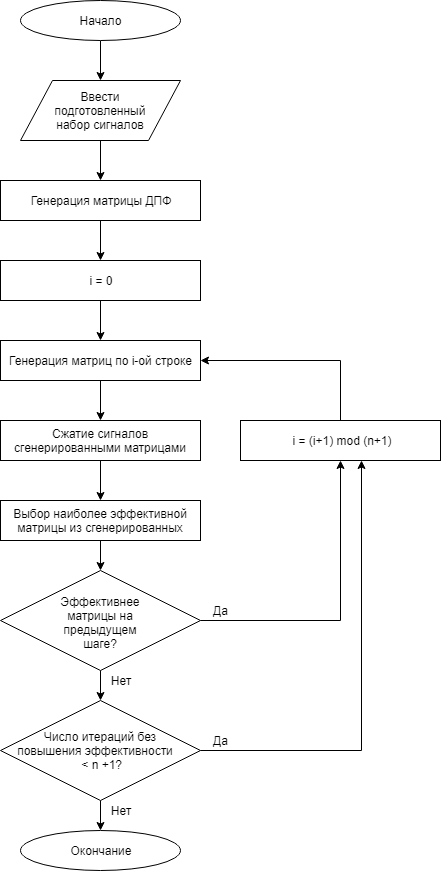
\includegraphics[scale=0.5]{block_diagram.png}}
	\caption{Блок-схема алгоритма}
	\label{block-diagram}
\end{figure}

\subsection{Выбор тестовых сигналов и уровня сжатия.}
Для решения поставленной задачи исследование проводится на наборе из $N=20$ сигналов $F_p$. Уровень сжатия выбран равным $80\%$. 

Поиск оптимального алгоритма сжатия имеет большую вычислительную сложность. В связи с этим на этапе предварительных расчетов для уменьшения количества операций рассматриваются сигналы, состоящие из $n+1=10$ отсчетов. 

В исследовании используются сигналы, которые представляют собой набор точек из QRS-комплекса электрокардиограммы(ЭКГ). Данный вид сигнала отражает изменение разницы электрических потенциалов активности сердца во времени и состоит из периодической последовательности кардиоциклов (рис. \ref{qsr-complex}). Одним из элементов такого цикла является QRS-комплекс, который отображает распространение возбуждения по желудочкам. Для проведения исследования были сняты ЭКГ с нескольких людей. Тестовые сигналы сгенерированы путем выбора из различных QRS-комплексов обозначенного ранее количества точек.

\begin{figure}[h]
	\center{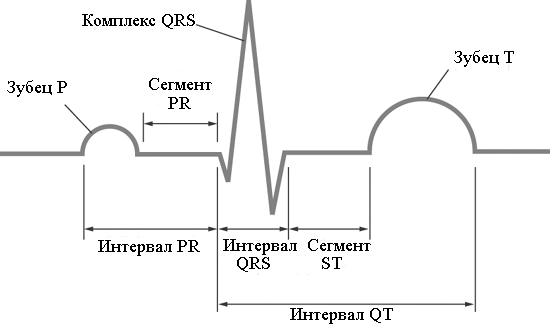
\includegraphics[scale=0.5]{qrs-complex.png}}
	\caption{Кардиоцикл ЭКГ}
	\label{qsr-complex}
\end{figure}

\subsection{Генерация матриц преобразования}

В качестве начального приближения была выбрана матрица дискретного косинусного преобразования Фурье (\ref{matrixDCT}), поскольку она дает достаточно хорошие результаты для широкого класса сигналов. Затем с каждым из элементов первой строки выполняется одно из 3-х действий: к нему прибавляется малая величина $\epsilon>0$, вычитается $\epsilon$, либо элемент остается неизменным (в наших расчетах $\epsilon=0,1$). В результате получается набор из $3^{n+1}$ матриц $S_q$, с которыми выполняются расчеты на всех дальнейших этапах.

Для каждой матрицы с помощью метода Гаусса находим обратную $T=S_q^{-1}$. В случае, если $S_q$ оказалась вырожденной, либо ее определитель близок к нулю, она исключается из дальнейшего рассмотрения, поскольку расчеты с участием плохо обусловленных матриц обладают известной вычислительной неустойчивостью [6, 7].

При повторном возвращении на этап генерации матриц преобразования производятся аналогичные действия со второй строкой, третьей и т. д. Затем весь процесс повторяется итерационно, пока не будут достигнуты условия завершения алгоритма. 

\subsection{Анализ, сжатие и синтез тестовых сигналов.}

На данном этапе последовательно перебираются матрицы $S_q$. С помощью каждой матрицы производится сжатия всех тестовых сигналов $F_p, p=1,2,...,N$. Обозначим $G_{qp}=S_q*F_p$. Далее производится обнуление части элементов векторов $G_{qp}$ в соответствии с выбранным уровнем сжатия. Новый набор векторов обозначим $\tilde{G_{qp}}$. После этого, применяя формулу (\ref{inverseConverstion}), получаем синтезированные сигналы $\tilde{F_{qp}}=T_q*\tilde{G_{qp}}$.

\subsection{Выбор наиболее эффективного преобразования.}

Для каждой матрицы $S_q$ рассматривается средняя по всему набору тестовых сигналов среднеквадратичная ошибка $<\sigma_q>$:
\begin{equation}
\label{squareNormQ}
    <\sigma_q> = \frac{\sum\limits_{p=1}^{N}||F_{qp}-\tilde{F_{qp}j}||}{N}
\end{equation}

Наиболее эффективным будем считать преобразование $S_q$, которое при заданном уровне сжатия дает наименьшее значение величины $<\sigma_q>$. В случае, если $S_q$ не позволяет достичь отклонения  меньшего, чем при использовании ДПФ, либо оно существенно не снизилось после проведения нескольких итераций, то алгоритм завершается. В противном случае следует вернуться к этапу генерации матриц преобразования, взяв за основу при дальнейших манипуляциях со строками найденную матрицу $S_q$

\section{Программная реализация алгоритма}

Реализация описанного выше алгоритма была выполнена на языке программирования C. Для ускорения работы программы была также использована технология OpenMP, позволяющая распараллелить программу на несколько потоков, работающих в системе с общей памятью. 

Разработанная реализация позволяет найти оптимальный алгоритм сжатия для подаваемого ей на вход набора сигналов. Выходными данными являются найденная, наиболее эффективная, матрица для преобразования сигналов, обратная к ней, а также отклонение по среднеквадратичной норме, полученное при сжатии сигналов вышеуказанной матрицей.

К настоящему моменту удалось добиться ускорения программы в $1,71$ раз, путём распределения по восьми потокам операций умножения сигналов на текущую матрицу преобразования. 

\section{Результаты расчётов}

Набор из $N = 100$ фрагментов ЭКГ был разбит на две равные группы. Одна из них использовалась для расчетов с использованием предложенного алгоритма, а вторая применялась для контроля эффективности сжатия. Параметр $\epsilon$ был выбран равным $0,1$.

Как показывают расчеты, найденное с помощью алгоритма преобразование в среднем демонстрирует более высокую эффективность на контрольном наборе сигналов, чем ДПФ. Например, в одном из экспериментов среднеквадратичная ошибка (\ref{squareNormQ}) при сжатии с помощью ДПФ составила величину $\approx25.0$, а  при использовании матрицы рассчитанного преобразования $\approx18.8$. Таким образом, удается получить алгоритм сжатия, который в среднем по эффективности выше или, по крайней мере, не уступает ДПФ.

Интерес представляет изучение того, насколько сильно результат будет зависеть от выбора начального приближения: вместо матрицы ДПФ могут быть использованы, например, вейвлеты. Это требует дополнительного исследования. 


\section{Заключение}

В ходе данной работы был разработан новый алгоритм поиска оптимального метода сжатия сигналов заданного. В связи с достаточно высокой вычислительной сложностью алгоритма, для его реализации используется суперкомпьютер. Ключевым достоинством предложенного подхода является, во-первых, универсальность: программа в автоматическом режиме должна осуществлять поиск наиболее эффективной матрицы преобразования. Во-вторых, простота реализации данного алгоритма.

Дальнейшее исследование будет посвящено изучению устойчивости алгоритма: насколько сильно зависит полученная матрица от состава и количества тестовых сигналов. Также планируется провести вычислительные эксперименты в ситуациях, когда вместо ДПФ в качестве начального приближения выбраны какие-либо матрицы, соответствующие различным вейвлет преобразованиям.


\section{Список литературы}

\begin{enumerate} 
\item Залманзон Л.А. Преобразования Фурье, Уолша, Хаара и их применение в управлении, связи и других областях / Л.А. Залманзон. – Москва: Наука, 1989. – 496 с.
\item Bracewell R. The Fourier Transform and its Applications. McGraw-Hill, 2000, 640 p.
\item Addison P. Wavelet Transforms and the ECG: a Review. Physiological Measurement, 2005, № 26(5), pp. R155–R199. DOI: 10.1088/0967-3334/26/5/R01.
\item Короновский А.А. Непрерывный вейвлетный анализ и его приложения / А.А. Короновский, А.Е. Храмов. – Москва: Физматлит, 2003. – 176 с.
\item Ватутин В.М. Алгоритм сжатия изображения с адаптацией базиса на каждом уровне вейвлет-пакетного разложения в информационно-управляющих системах для визуального контроля управляемого объекта / В.М. Ватутин [и др.] // Информационно-измерительные и управляющие системы. – 2007. – Т. 5, № 7. – С. 37–40.
\item Воронкин Р.А. Сжатие изображений с помощью адаптивных ортогональных вейвлетов четвертого порядка и генетических алгоритмов / Р.А. Воронкин // Информационно-измерительные и управляющие системы. – 2014. – № 2. – С. 83–87.
\item Никифоров П.Л. Модель электрокардиографического сигнала на основе совокупности колокольных импульсов / П.Л. Никифоров // Вестник молодых ученых. Серия технически науки. – 1998. – № 1. – С. 64–68.
\item Киселев Е.А. Комбинированный алгоритм сжатия сигнала электрокардиограммы с помощью всплесков Добеши и функции Гаусса / Е.А. Киселев, Насер Нихад Махмуд, Е.Г. Супонев // Системы управления и информационные технологии. – 2017, № 3(69). – С. 53–56.

\end{enumerate}

\end{document}